\documentclass{../../note}

\usepackage{amsthm}
\usepackage{pgfplots}
\pgfplotsset{compat=1.18}
\newtheorem{example}{Example}

\title{数据结构 01}
\author{isomo}

\begin{document}

\maketitle

\section{绪论}

\subsection{引言}
数据结构是计算机科学中的一门基础课程,它研究数据的组织方式及其操作,对于程序设计、算法设计和计算机系统设计都有着重要的影响。本章将介绍数据结构的基本概念,包括数据、数据元素、数据结构、数据类型、抽象数据类型等,同时也会讨论算法及其分析方法。

\subsection{数据及相关概念}

\subsubsection{数据的概念}
\begin{itemize}
  \item \textbf{数据}(Data):是对客观事物的符号表示,在计算机科学中,是指所有能输入到计算机中并被计算机程序处理的符号的总称。
  \item 数据是计算机程序加工的原料,是信息的载体。
  \item 数据可以是数值型(如1, 2, 3.14等)、文本型(如"Hello")、图形型、音频型等多种形式。
\end{itemize}

\begin{example}
  学生信息系统中的学生姓名、学号、成绩等都是数据。
  天气预报系统中的温度、湿度、气压等也是数据。
\end{example}

\subsubsection{数据元素的概念}
\begin{itemize}
  \item \textbf{数据元素}(Data Element):是数据的基本单位,通常作为一个整体进行考虑。
  \item 也称为记录(Record)、节点(Node)或实体(Entity)。
  \item 一个数据元素可由若干个数据项(Data Item)组成。
\end{itemize}

\begin{example}
  在学生信息系统中,每个学生的完整信息(包括姓名、学号、成绩等)构成一个数据元素。
  在图书管理系统中,每本书的信息(包括书名、作者、ISBN等)是一个数据元素。
\end{example}

\subsubsection{数据项的概念}
\begin{itemize}
  \item \textbf{数据项}(Data Item):是数据的最小单位,是不可分割的基本单位。
  \item 数据项是组成数据元素的基本单位。
\end{itemize}

\begin{example}
  学生信息中的姓名是一个数据项,学号是一个数据项,成绩是一个数据项。
\end{example}

\subsection{数据结构}

\subsubsection{数据结构的定义}
\begin{itemize}
  \item \textbf{数据结构}(Data Structure):是相互之间存在一种或多种特定关系的数据元素的集合。
  \item 数据结构包括三个方面:
    \begin{enumerate}
      \item 数据的逻辑结构
      \item 数据的存储结构(物理结构)
      \item 数据的操作
    \end{enumerate}
\end{itemize}

\subsubsection{数据的逻辑结构}
\begin{itemize}
  \item \textbf{逻辑结构}(Logical Structure):指数据元素之间的逻辑关系,与数据的存储无关。
  \item 主要分为以下四类:
    \begin{enumerate}
      \item \textbf{线性结构}:元素之间是一对一的关系。如线性表、栈、队列等。
      \item \textbf{树形结构}:元素之间是一对多的关系。如树、二叉树等。
      \item \textbf{图形结构}:元素之间是多对多的关系。如图、网络等。
      \item \textbf{集合结构}:元素之间除了同属一个集合外,没有其他关系。
    \end{enumerate}
\end{itemize}

\begin{figure}[h]
  \centering
  \begin{tikzpicture}
    \node[draw, rectangle] (a) at (0,0) {逻辑结构};
    \node[draw, rectangle] (b1) at (-3,-1.5) {线性结构};
    \node[draw, rectangle] (b2) at (-1,-1.5) {树形结构};
    \node[draw, rectangle] (b3) at (1,-1.5) {图形结构};
    \node[draw, rectangle] (b4) at (3,-1.5) {集合结构};

    \draw[->] (a) -- (b1);
    \draw[->] (a) -- (b2);
    \draw[->] (a) -- (b3);
    \draw[->] (a) -- (b4);
  \end{tikzpicture}
  \caption{数据的逻辑结构分类}
\end{figure}

\subsubsection{数据的存储结构}
\begin{itemize}
  \item \textbf{存储结构}(Storage Structure):指数据在计算机中的表示(又称物理结构)。
  \item 存储结构是逻辑结构在计算机中的映射,通过存储单元之间的邻接关系来反映数据元素之间的逻辑关系。
  \item 主要分为以下四类:
    \begin{enumerate}
      \item \textbf{顺序存储结构}:使用一组地址连续的存储单元依次存储数据元素。
      \item \textbf{链式存储结构}:使用一组任意的存储单元存储数据元素,每个元素还存储指向相关元素的指针。
      \item \textbf{索引存储结构}:在存储数据的同时,建立附加的索引表,以便快速访问。
      \item \textbf{散列存储结构}:根据数据元素的关键字直接计算其存储地址。
    \end{enumerate}
\end{itemize}

\begin{figure}[h]
  \centering
  \begin{tikzpicture}
    \node[draw, rectangle] (a) at (0,0) {存储结构};
    \node[draw, rectangle] (b1) at (-3,-1.5) {顺序存储};
    \node[draw, rectangle] (b2) at (-1,-1.5) {链式存储};
    \node[draw, rectangle] (b3) at (1,-1.5) {索引存储};
    \node[draw, rectangle] (b4) at (3,-1.5) {散列存储};

    \draw[->] (a) -- (b1);
    \draw[->] (a) -- (b2);
    \draw[->] (a) -- (b3);
    \draw[->] (a) -- (b4);
  \end{tikzpicture}
  \caption{数据的存储结构分类}
\end{figure}

\subsection{数据类型与抽象数据类型}

\subsubsection{数据类型}
\begin{itemize}
  \item \textbf{数据类型}(Data Type):是一组性质相同的值的集合及定义在此集合上的一组操作的总称。
  \item 数据类型可以分为两类:
    \begin{enumerate}
      \item \textbf{原子类型}(基本类型):不可再分的类型,如整数、实数、字符等。
      \item \textbf{结构类型}:由多个类型组合而成,如数组、结构体等。
    \end{enumerate}
  \item 在编程语言中,声明变量时必须指定数据类型,如int、float、char等。
\end{itemize}

\subsubsection{抽象数据类型}
\begin{itemize}
  \item \textbf{抽象数据类型}(Abstract Data Type, ADT):是一个数学模型及定义在该模型上的一组操作,它与存储结构的实现无关。
  \item ADT由两部分组成:
    \begin{enumerate}
      \item 数据对象的抽象描述
      \item 对数据对象的操作的抽象描述
    \end{enumerate}
  \item ADT的表示方法:
    \begin{verbatim}
    ADT 抽象数据类型名 {
        数据对象: <数据对象的定义>
        数据关系: <数据关系的定义>
        基本操作: <基本操作的定义>
    }
    \end{verbatim}
\end{itemize}

\begin{example}[抽象数据类型示例]
  以"线性表"为例,其ADT可表示为:
\begin{verbatim}
ADT List {
    数据对象:
        D = {a_i | a_i ∈ ElemSet, i = 1, 2, ..., n, n ≥ 0}
    数据关系:
        R = {<a_i, a_{i+1}> | a_i, a_{i+1} ∈ D, i = 1, 2, ..., n-1}
    基本操作:
        InitList(&L)   // 初始化线性表
        Length(L)      // 求表长
        GetElem(L, i, &e)  // 获取第i个元素
        LocateElem(L, e)   // 查找元素e的位置
        Insert(&L, i, e)   // 在位置i插入元素e
        Delete(&L, i, &e)  // 删除位置i的元素
        ...
}
\end{verbatim}
\end{example}

\subsection{算法及其分析}

\subsubsection{算法的概念}
\begin{itemize}
  \item \textbf{算法}(Algorithm):是解决特定问题的一系列操作的有限序列。
  \item 算法的五个基本特性:
    \begin{enumerate}
      \item \textbf{有穷性}:算法必须在有限步骤内结束。
      \item \textbf{确定性}:算法的每一步骤必须有确定的含义,不能有歧义。
      \item \textbf{可行性}:算法的每一步操作都必须是可行的,即能够通过已经实现的基本操作执行有限次来实现。
      \item \textbf{输入}:算法可以有零个或多个输入。
      \item \textbf{输出}:算法必须有一个或多个输出。
    \end{enumerate}
\end{itemize}

\subsubsection{算法的描述}
算法可以通过多种方式描述:
\begin{enumerate}
  \item \textbf{自然语言}:使用日常语言描述算法步骤。
  \item \textbf{流程图}:使用图形符号表示算法的流程。
  \item \textbf{伪代码}:介于自然语言和程序设计语言之间的描述方式。
  \item \textbf{程序设计语言}:如C、Java等。
\end{enumerate}

\begin{example}[简单算法示例:顺序查找]
  伪代码描述:
\begin{verbatim}
Algorithm SequentialSearch(A[0...n-1], key):
    i = 0
    while i < n and A[i] != key do
        i = i + 1
    if i < n then
        return i  // 找到元素,返回位置
    else
        return -1 // 未找到元素,返回-1
\end{verbatim}
\end{example}

\subsubsection{算法的分析}
算法分析的两个主要方面:
\begin{enumerate}
  \item \textbf{正确性分析}:证明算法是否能正确地解决问题。
  \item \textbf{效率分析}:评估算法的时间复杂度和空间复杂度。
    \begin{itemize}
      \item \textbf{时间复杂度}:算法执行所需的时间。
      \item \textbf{空间复杂度}:算法执行所需的存储空间。
    \end{itemize}
\end{enumerate}

\paragraph{渐进符号}
用于表示算法时间复杂度的常用符号:
\begin{itemize}
  \item \textbf{O(大O)}:表示上界,如O(n²)表示算法的执行时间不超过n²的常数倍。
  \item \textbf{Ω(大Omega)}:表示下界,如Ω(n)表示算法的执行时间至少是n的常数倍。
  \item \textbf{Θ(大Theta)}:表示确界,如Θ(n)表示算法的执行时间恰好是n的常数倍。
\end{itemize}

\paragraph{常见的时间复杂度}
按照效率从高到低排序:
\begin{itemize}
  \item O(1):常数时间,与输入规模无关。
  \item O(log n):对数时间,如二分查找。
  \item O(n):线性时间,如顺序查找。
  \item O(n log n):线性对数时间,如归并排序、快速排序。
  \item O(n²):平方时间,如冒泡排序、插入排序。
  \item O(n³):立方时间,如某些矩阵运算。
  \item O($2^n$):指数时间,如穷举法。
\end{itemize}

\begin{figure}[h]
  \centering
  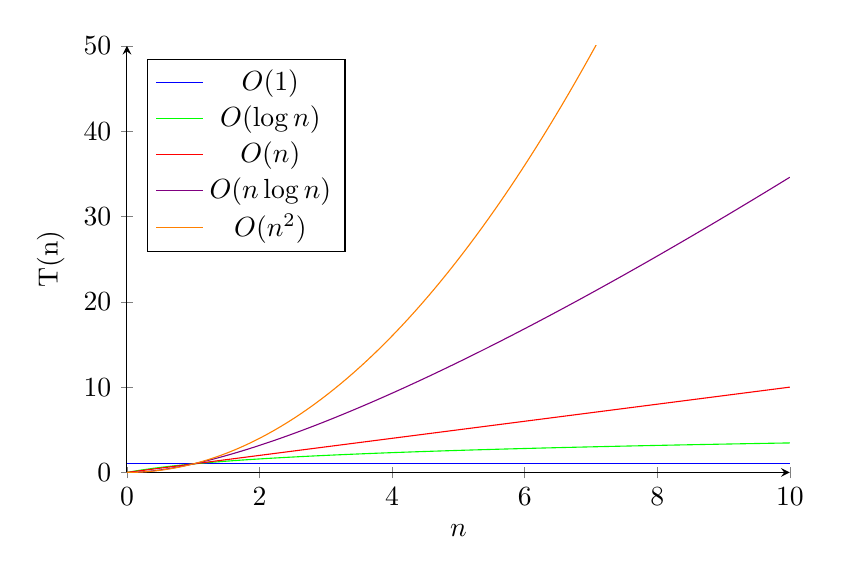
\begin{tikzpicture}
    \begin{axis}[
        domain=0:10,
        samples=100,
        axis lines=left,
        xlabel={$n$},
        ylabel={T(n)},
        legend pos=north west,
        width=10cm,
        height=7cm,
        ymax=50,
      ]
      \addplot[color=blue] {1};
      \addlegendentry{$O(1)$}

      \addplot[color=green] {ln(x+1)/ln(2)};
      \addlegendentry{$O(\log n)$}

      \addplot[color=red] {x};
      \addlegendentry{$O(n)$}

      \addplot[color=violet] {x*ln(x+1)/ln(2)};
      \addlegendentry{$O(n \log n)$}

      \addplot[color=orange] {x^2};
      \addlegendentry{$O(n^2)$}

    \end{axis}
  \end{tikzpicture}
  \caption{常见时间复杂度函数的增长趋势}
\end{figure}

\paragraph{算法效率分析实例}
\begin{example}[顺序查找算法的时间复杂度分析]
  顺序查找算法的最坏情况:要查找的元素在数组的最后或不存在,需要比较n次,时间复杂度为O(n)。
  最好情况:要查找的元素在数组的第一个位置,只需比较1次,时间复杂度为O(1)。
  平均情况:假设查找任意位置的概率相等,则平均需要比较(n+1)/2次,时间复杂度仍为O(n)。
\end{example}

\subsection{数据结构的应用}

数据结构在计算机科学和实际应用中具有广泛的应用:

\begin{itemize}
  \item \textbf{数据库系统}:利用各种数据结构组织和存储数据,实现高效的数据管理。
  \item \textbf{操作系统}:利用队列管理进程,利用树结构管理文件系统等。
  \item \textbf{编译器}:利用栈实现表达式求值,利用树结构表示语法分析等。
  \item \textbf{搜索引擎}:利用倒排索引等数据结构实现高效的信息检索。
  \item \textbf{图形处理}:利用图和树等结构描述图像和几何对象的关系。
  \item \textbf{人工智能}:利用各种数据结构表示知识和实现搜索算法。
\end{itemize}

\subsection{本章小结}
本章介绍了数据结构的基本概念,包括数据、数据元素、数据项、数据的逻辑结构和存储结构、数据类型和抽象数据类型等。同时,也讨论了算法的概念、算法的描述方法以及算法分析的基本方法,特别是时间复杂度和空间复杂度的概念和分析方法。这些基础知识是学习后续各种具体数据结构和算法的必要前提。

\section{线性表}

\end{document}